\documentclass[a4paper]{article}
\usepackage{graphicx}
\usepackage[bookmarks=true]{hyperref}
\usepackage{bookmark}
\usepackage[margin=1.2in]{geometry}
\usepackage{float}
\usepackage{caption}
\usepackage{hyperref}
\usepackage[english]{babel}
\usepackage{graphicx}

\title{Functional Requirements}
\author{The Baobab Team}

\begin{document}

\newpage
\begin{titlepage}

\begin{center}


\includegraphics[width=400px]{pictures/logo.jpg}
\vspace{0.5 cm}
\begin{flushright} \large
\begin{tabular}{lr}
\vspace{1 cm}
\LARGE\textbf{Document:}Sprint Report 6\\

\vspace{1 cm}
\LARGE\textbf{Project:} Group Chat For Linphone (Agile DO-178)\\
\vspace{1 cm}
\LARGE\textbf{Advisor:} Kobus Coetzee\\
\vspace{1 cm}
\LARGE\textbf{Sponsors:} Nanoteq \& Department of Computer Science, UP\\
\vspace{1 cm}
\LARGE\textbf{Date: }\today\\
\end{tabular}
\end{flushright}

\centering 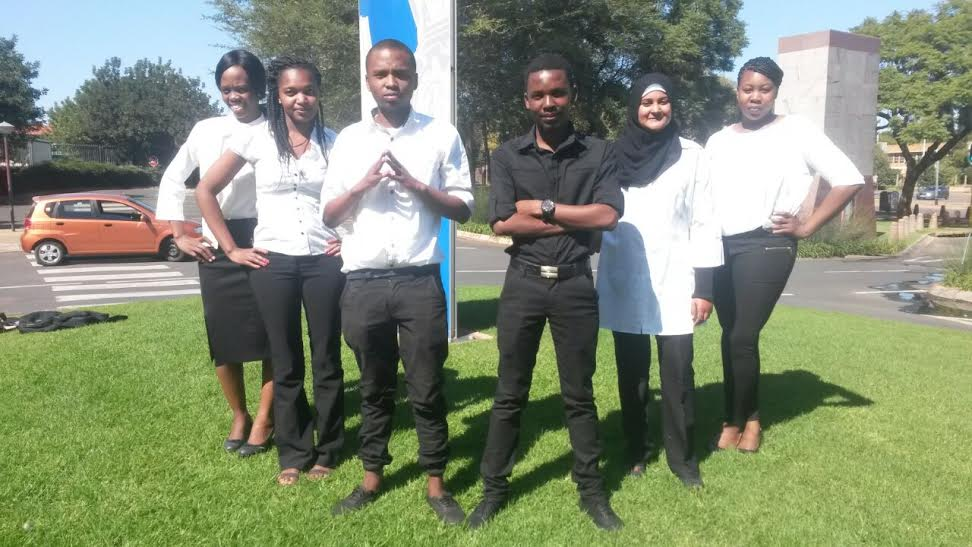
\includegraphics[width=350px]{pictures/Team.jpg}

Patience Mtsweni, Lerato Molokomme, Tsepo Ntsaba, Mpedi Mello, Lutfiyya Razak, Ephiphania Munava\\


\end{center}
\end{titlepage}

\newpage
\begin{center}
\LARGE \textbf{Member details}\\
\begin{tabular}{ll}
Ephiphania Munava&10624610\\
Lutfiyya Razak&10198408\\
Lerato Molokomme&11197961\\
Mpedi Mello&11210754\\
Patience Mtsweni&11116774\\
Tsepo Ntsaba&10668544\\

\end{tabular}
\end{center}

\newpage
\tableofcontents
\listoffigures
\newpage

\section{\textbf{\huge{Introduction}}}
\subsection{Purpose}
The purpose of this project is to extend Linphone's Instant Messaging (IM) implementation on Android platforms to include group chat and to implement other minor improvements to Linphones IM capabilities and user interface. 

\subsection{Scope}
We are required to develop the following functionality for the Linphone project:
\begin{itemize}
\item Group chat (Invite additional members to a chat, all members receive chats)
\item Secure group chat (AES256)
\item Creation and deletion of groups
\item Voice record and send over IM
\item Improve the messaging user interface
	\begin{itemize}
		\item Spacing between words are terrible
		\item Make text bigger
		\item Blocks indents required to better specify who said what
		\item Presence indication to show a remote user is typing
		\item User picture portraits
	\end{itemize}
\end{itemize}

%Overview
\section{\textbf{\huge{Overview of Linphone Group Chat}}}
\large{Diagram to show an abstract overview of the Linphone Group Chat. This system will be discussed in greater detail in the rest of the article.}\\
\begin{figure}[H]
\centering
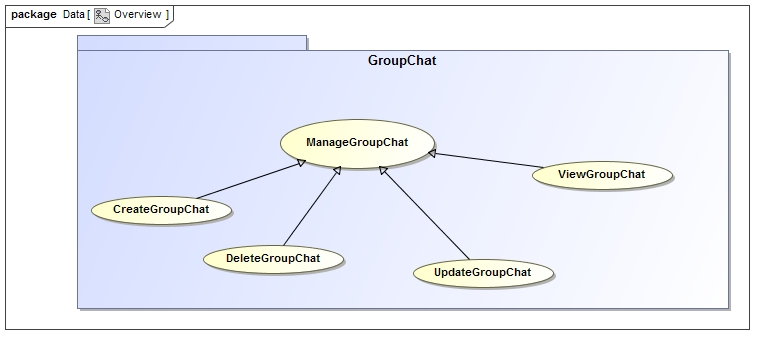
\includegraphics[width=1\linewidth]{./pictures/Overview.jpg}
\caption{Overview of Linphone group chat}
\end{figure}
\newpage


%Linphone group chat
\section{\textbf{\huge{Linphone Group Chat}}}

%CREATE GROUP CHAT
\subsection{Create Group Chat}
\subsubsection{Required Functionality:} 
\begin{figure}[H]
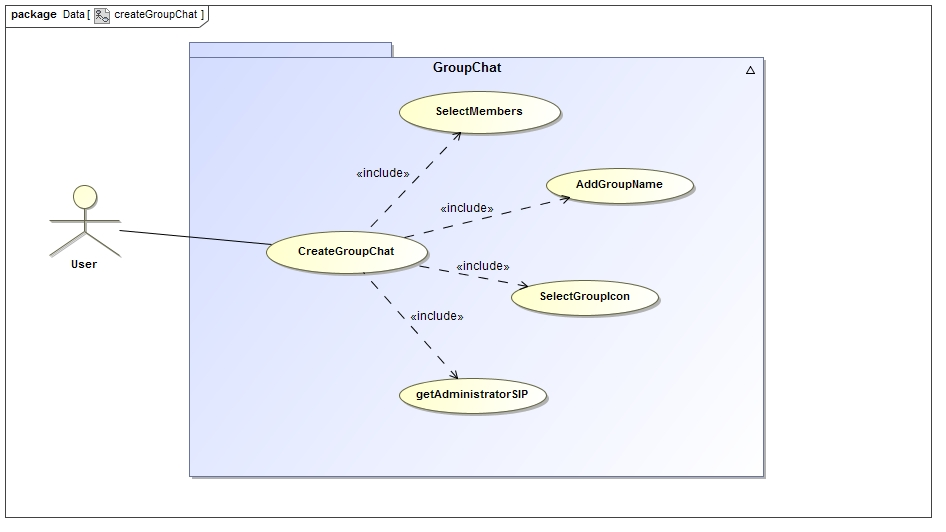
\includegraphics[width=1\linewidth]{./pictures/createGroupChat.jpg}
\caption{Create Group Chat use case diagram}
\end{figure}

\textbf{Description:}This use case encapsulates the ability for a user to create a new group chat. Upon the creation of the group chat, the user will have the group chat appear on thier chats screen. The user will now be able to chat with other group members.

\subsubsection{Prioritization:}Critical
\subsubsection{Conditions and Data Structures:}
\textbf{Pre-Conditions:}
\begin{itemize}
	\item The user wanting to create a new group chat should register on linphone and have a registered account.
	\item The user should have the people that they want to add to the group chat as contacts on their linphone application. 
		  The participants to be added should also have a registered linphone account.
\end{itemize}
\textbf{Post-Conditions:}
\begin{itemize}
	\item A message is displayed to inform the creator of the group chat that the creation has been successful. Users can now chat in the group.
	\item If this service has been rejected, an exception is thrown and an error message will be displayed to the user.
\end{itemize}
	
\subsubsection{Process Specifications:} 
\begin{figure}[H]
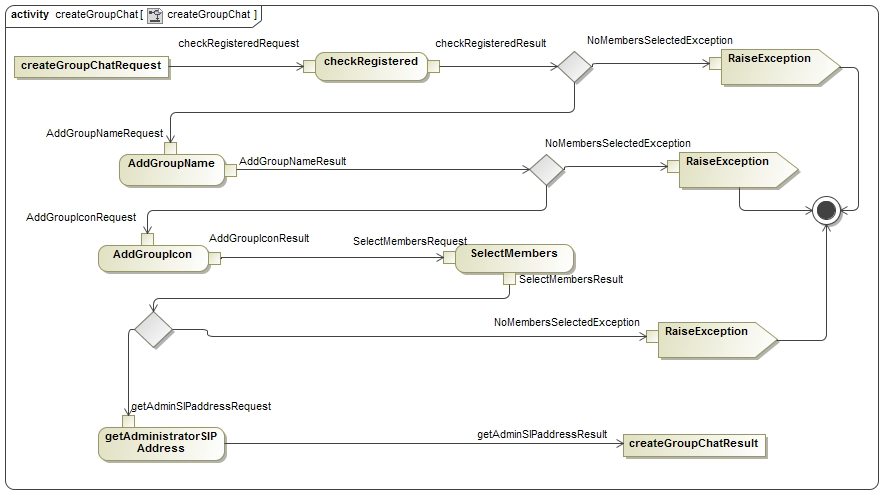
\includegraphics[width=1\linewidth]{./pictures/create_GroupChat.jpg}
\caption{Create Group Chat activity diagram }
\end{figure}

\subsection{Domain model}
This is the domain model for the group chat
\begin{figure}[H]
\centering
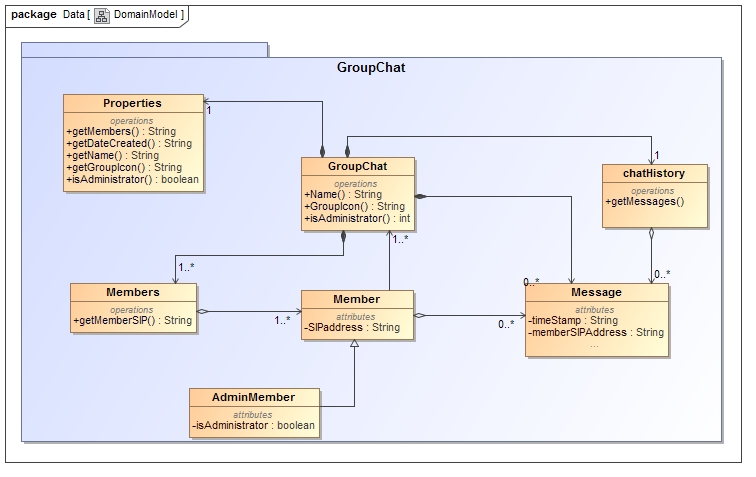
\includegraphics[width=1\linewidth]{./pictures/DomainModel.jpg}
\caption{Domain model for Group Chat}
\end{figure}

Note that the relationship between the GroupChat and Properties,Members, Message and chatHistory is a composite relationship because they are only accessible from the GroupChat and if the GroupChat is deleted, they all are also deleted.\\
\\
There is a aggregation relationship between Members and member because the members class has to consists of one or more members. \\
\\
There is also a specialization relationship between member and AdminMember because a member can be administrator member(can add members, remove members,delete group) or a basic group member(can edit group icon,group name and view members).
\end{document}